
\documentclass[10pt,xcolor=table]{beamer}
\usepackage[french]{babel}
\usepackage[T1]{fontenc}
\usepackage[utf8]{inputenc}
\usetheme{Warsaw}
\usepackage{pdfpages}


\begin{document}
%nico la pute 
\begin{frame}
  \frametitle{Introduction}

  \begin{itemize}[<+->]
  \item La Stéganographie,
  \item 16ème siècle avant J-C,
  \item Ronald Rivest et le cryptage RSA
  
  \begin{block}{Les 3 critères}
    \begin{itemize}
    \item Confidentialité,
    \item Authenticité,
    \item integrité
    \end{itemize}
  \end{block}
  \end{itemize}
  \pause
  \begin{center}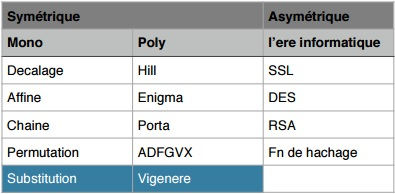
\includegraphics[scale=0.4]{Tab1.jpg}\end{center}

\end{frame}

\section{Développement}

\begin{frame}[<+->]
  \frametitle{Développement}
  
  \begin{exampleblock}{Produit sur le marché}
	\begin{enumerate}
    \item www.decode.fr,
    \item Decrypto (Google Play Store),
    \item Axcypte
    \end{enumerate}
  \end{exampleblock}

  \begin{block}{Phase de développement}
   
    \begin{enumerate}
    \item Identification,
    \item Définition,
    \item Réalisation,
    \item Finalisation
    \end{enumerate}
  \end{block}

\end{frame}
%younes
\begin{frame}
\begin{exampleblock}{Un exemple de cryptage} % Bloc exemple vert
\rowcolors{1}{blue!20}{blue!10} 
\begin{tabular}{l!{\vrule}ccccccc} 
text clair & A & T & T & A & Q & U & E \pause \\  
equivalent entier & 0 & 19 & 19 & 0 & 16 & 20 & 4 \pause \\ 
cle & B & U & T & B & U & T & B \pause  \\ 
equivalent entier & 1 & 20 & 19 & 1 & 20 & 19 & 1\pause \\ \hline
la somme & 1 & 39 & 38 & 1 & 36 & 39 & 5\pause \\ \hline
modulo 26 & 1 & 13 & 12 & 1 & 10 & 13 & 5 \pause \\ \hline
text crypté & B & N & M & B & K & N & F \pause \\
\end{tabular}
\end{exampleblock}
\begin{exampleblock}{Un exemple de decryptage (partie 1)} % Bloc exemple vert
 CHREEVOAHMAERATBIAXXWTNXBEEOPHBSBQMQEQERBWRVX
 UOAKXAOSXXWEAHBWEJMNQMNKERFVEXWTRZXWIAKLXFPSK
 AUTEMNDCMGTSXMXBTUIADNGMGPSRELXNIELXVRVPRTULH
 DNQWTWDTYGBPMXTFALJHASVBFXNGLLCHRZBWELEKMSSIK
 NBHWRIGNMGJSGLXFEYPHAGNRBIEQJTAMRVLCRREMNDGLX
 RRIMGNSNRVCHRQHAEYEVTAQEBBIPEEWEVKAKOEWADREMX
 MTBHHCHRTKDNVRZCHRCLQOHPWQAIIWXNRMGVOIIFKEE
\end{exampleblock}
\end{frame}
\begin{frame}

\begin{exampleblock}{Un exemple de cryptage} % Bloc exemple vert
\rowcolors{1}{blue!20}{blue!10} 
\begin{tabular}{l!{\vrule}ccccccc} 
text clair & A & T & T & A & Q & U & E \\  
equivalent entier & 0 & 19 & 19 & 0 & 16 & 20 & 4 \\ 
cle & B & U & T & B & U & T & B \\ 
equivalent entier & 1 & 20 & 19 & 1 & 20 & 19 & 1\\ \hline
la somme & 1 & 39 & 38 & 1 & 36 & 39 & 5 \\ \hline
modulo 26 & 1 & 13 & 12 & 1 & 10 & 13 & 5  \\ \hline
text crypté & B & N & M & B & K & N & F  \\
\end{tabular}
\end{exampleblock}
\begin{exampleblock}{Un exemple de decryptage (partie 1)} % Bloc exemple vert
 \textcolor{red}{CHR}EEVOAHMAERATBIAXXWTNXBEEOPHBSBQMQEQERBWRVX
 UOAKXAOSXXWEAHBWEJMNQMNKERFVEXWTRZXWIAKLXFPSK
 AUTEMNDCMGTSXMXBTUIADNGMGPSRELXNIELXVRVPRTULH
 DNQWTWDTYGBPMXTFALJHASVBFXNGLL\textcolor{red}{CHR}ZBWELEKMSSIK
 NBHWRIGNMGJSGLXFEYPHAGNRBIEQJTAMRVLCRREMNDGLX
 RRIMGNSNRV\textcolor{red}{CHR}QHAEYEVTAQEBBIPEEWEVKAKOEWADREMX
 MTBHHCHRTKDNVRZ\textcolor{red}{CHR}CLQOHPWQAIIWXNRMGVOIIFKEE\\ \pause
 Distances : 165 ,235 et 285 \\ \pause
 PGCD (165,235,285) = 5 
\end{exampleblock}
\end{frame}

\begin{frame}

\begin{exampleblock}{Un exemple de decryptage (partie 2)} % Bloc exemple vert
$M_{g} = \sum_{i=0}^{25} \frac{P_{i} F_{i+g}}{n^{'}}$\\ \pause
\rowcolors{1}{blue!20}{blue!10} 
\tabcolsep=3pt
\begin{tabular}{l!{\vrule}cccccccccccccc} 
text crypté & C & H & R & E & E & V & O & A & H & M & A & E & R \pause \\  
equivalent entier & 2 & 7 & 17 & 4 & 4 & 21 & 14 & 0 & 7 & 12 & 0 & 4 & 17 \pause \\ 
cle & J & A & N &  E & T & J & A & N &  E & T & J & A & N  \pause  \\ 
equivalent entier & 9 & 0 & 13 & 4 & 19 & 9 & 0 & 13 & 4 & 19 & 9 & 0 & 13\pause \\ \hline
la difference & -7 & 7 & 4 & 0 & -15 & 12 & 14 & -13 & 3 & -7 & -9 & 4 & 4 \pause \\ \hline
modulo 26 & 19 & 7 & 4 & 0 & 11 & 12 & 14 & 13 & 3 & 19 & 17 & 4 & 4 \pause \\ \hline
text clair & T & H & E & A & L & M & O & N & D & T & R & E & E \pause \\
\end{tabular}
\end{exampleblock}
\end{frame}
%tibo
\begin{frame}
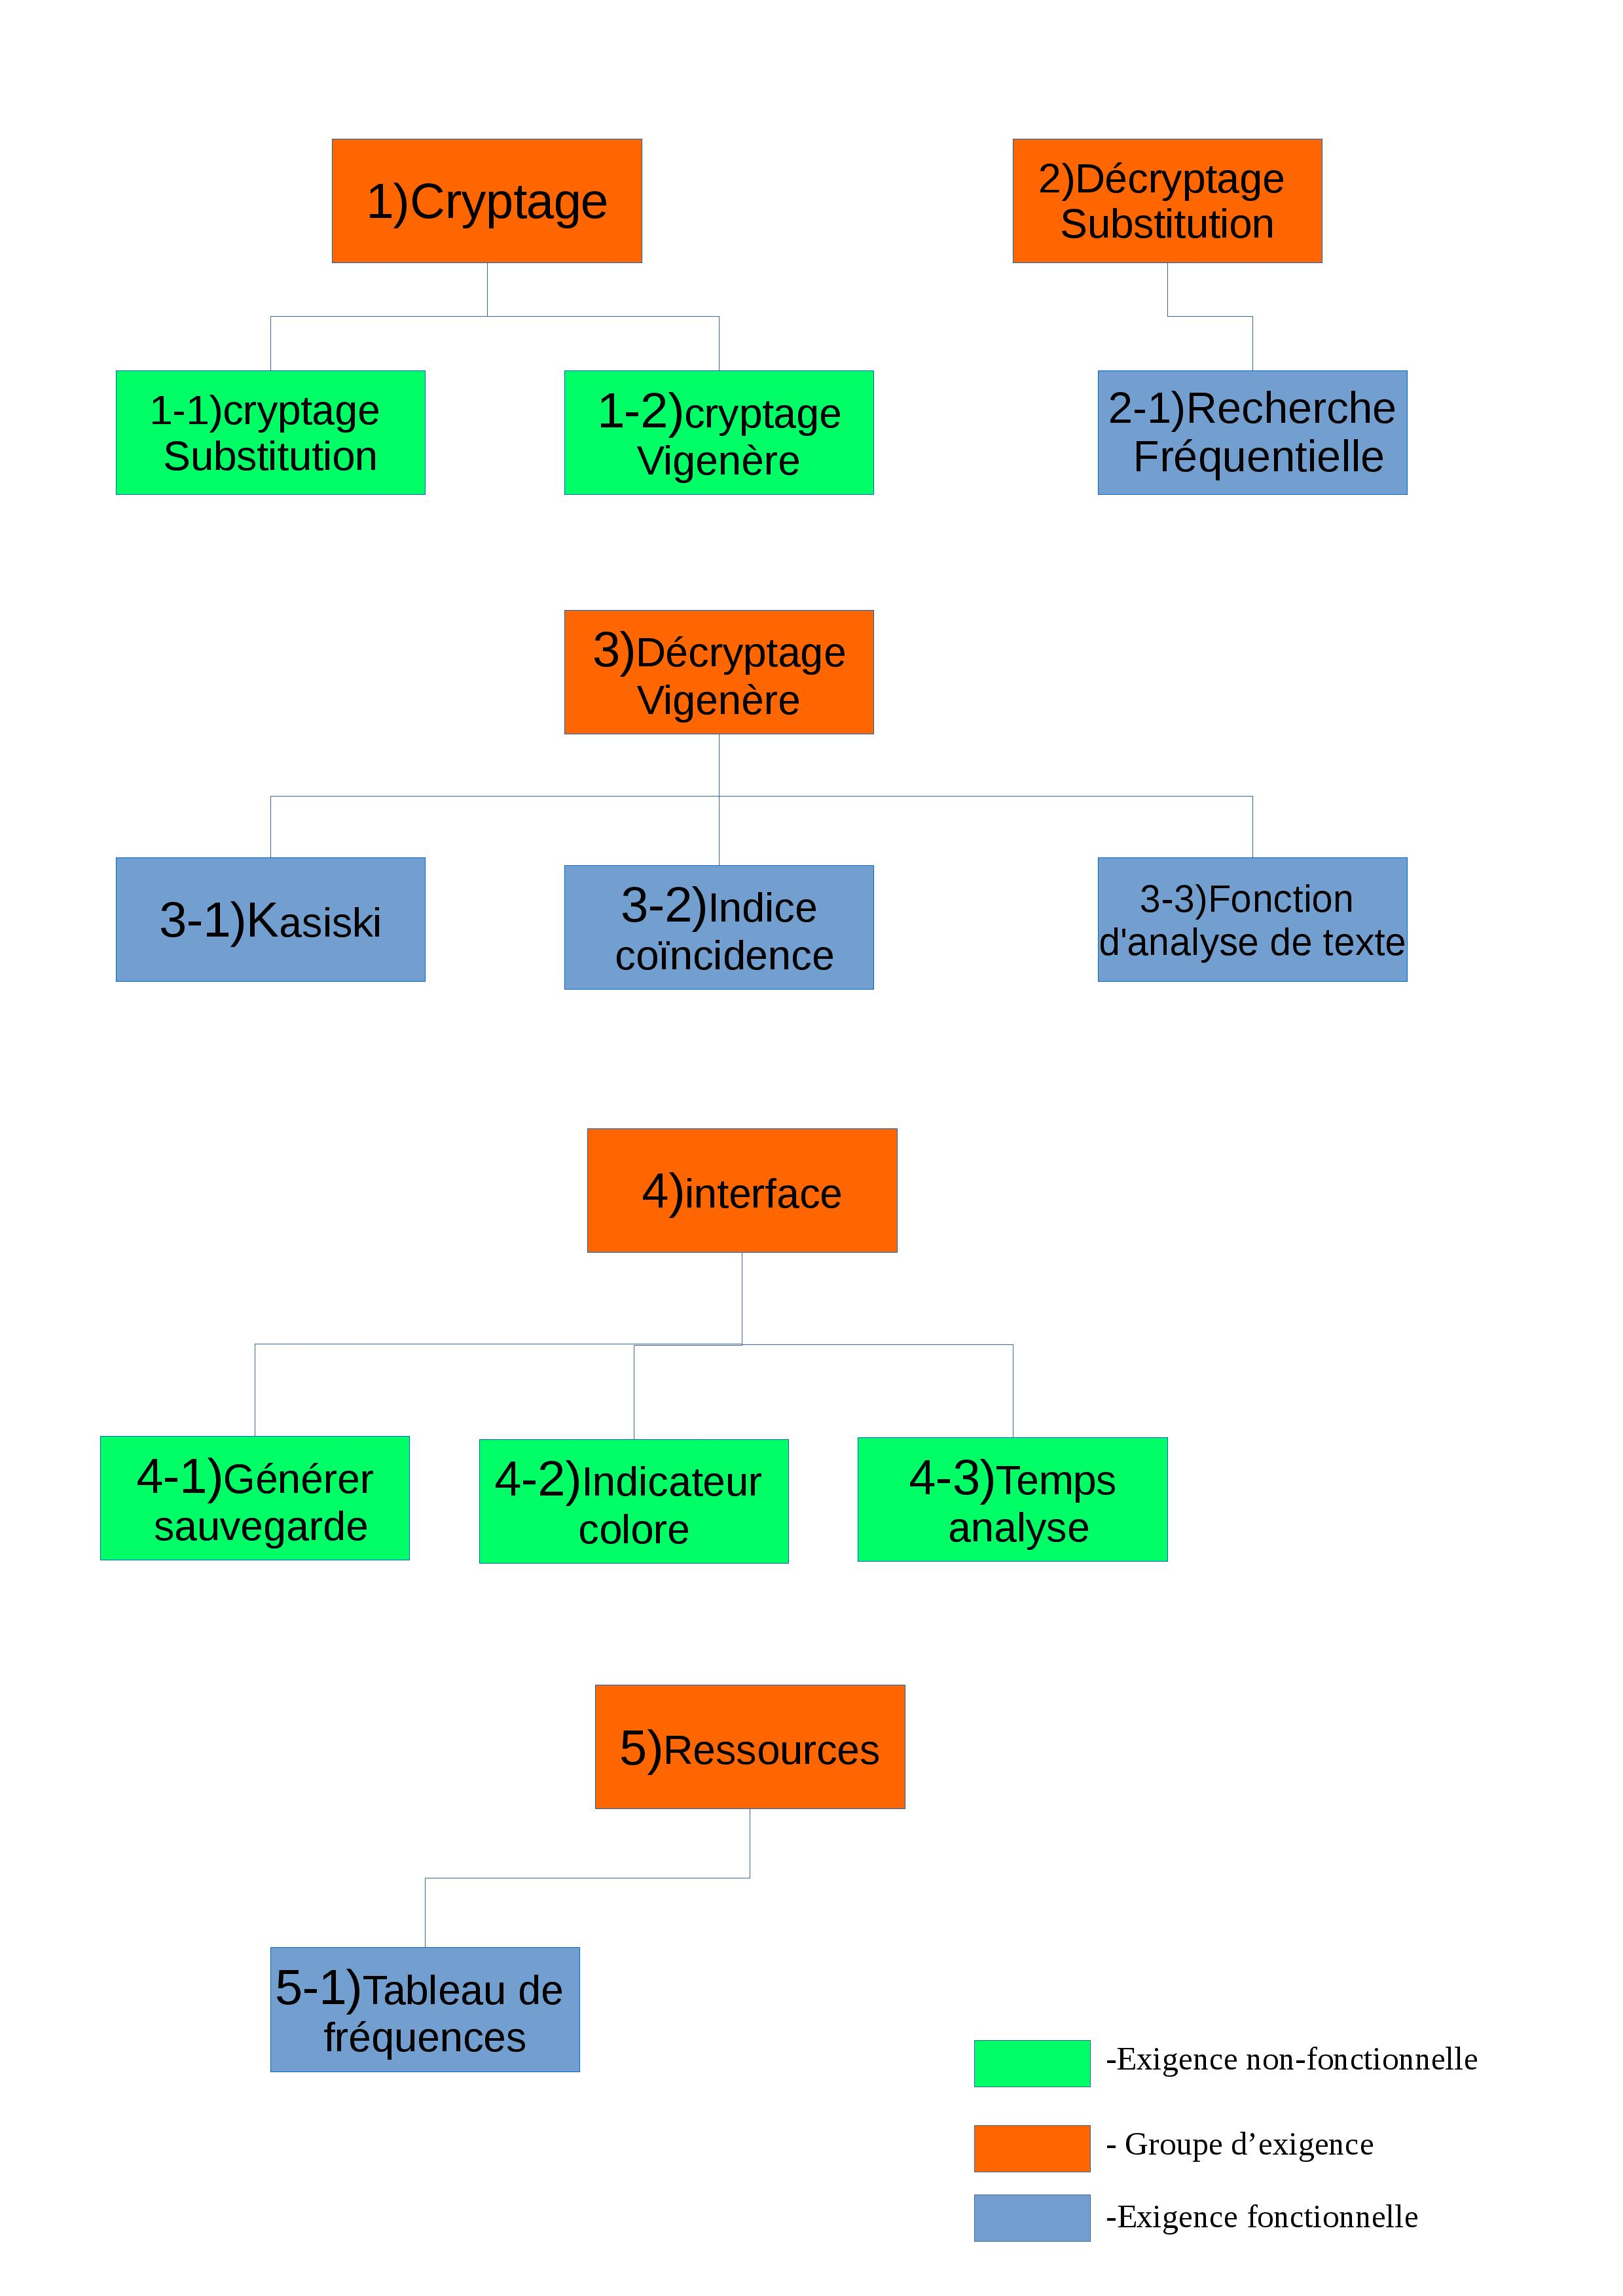
\includegraphics[scale = 0.2]{Arbr.jpg} \pause 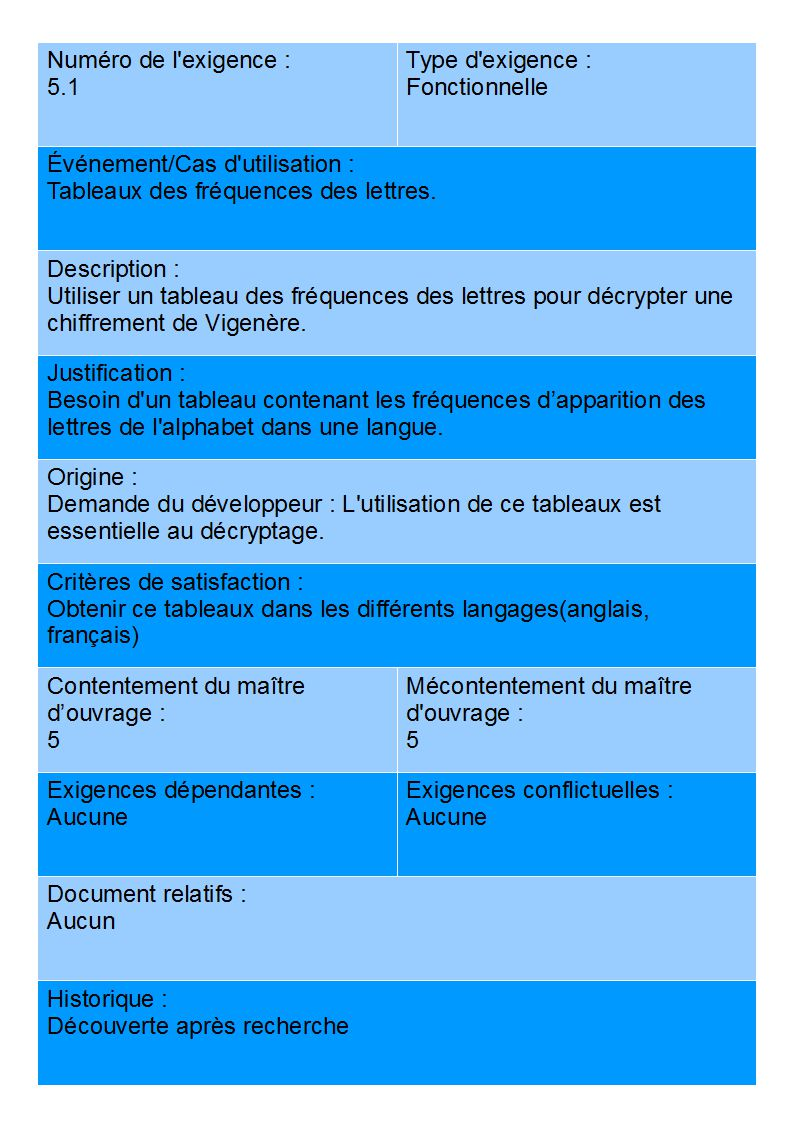
\includegraphics[scale = 0.5]{tab-freq.jpg} \pause 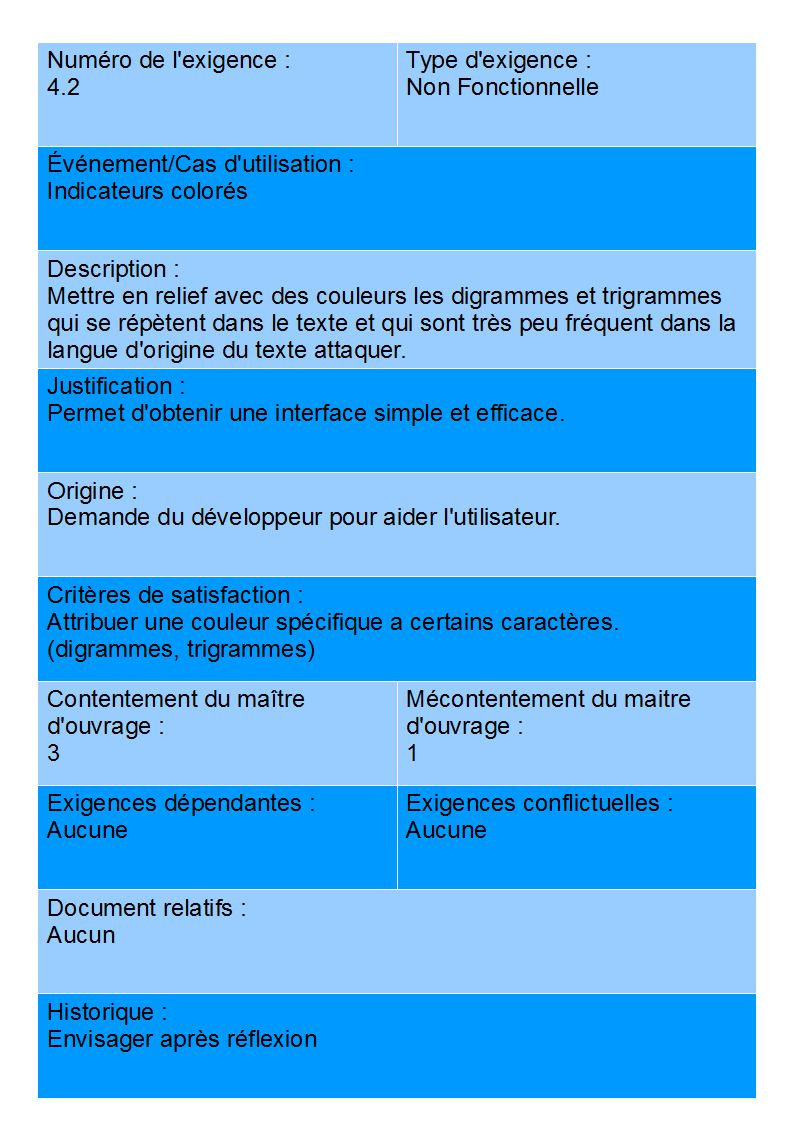
\includegraphics[scale = 0.5]{color.jpg}
\end{frame}
\begin{frame}
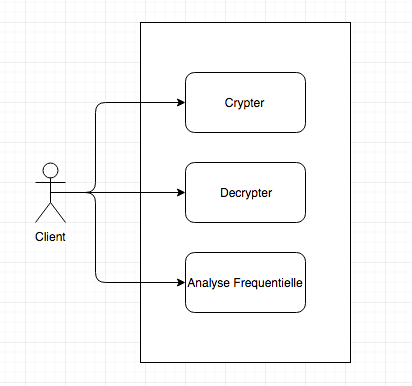
\includegraphics[scale = 0.5]{dia.png}
\end{frame}
%flo
\begin{frame}
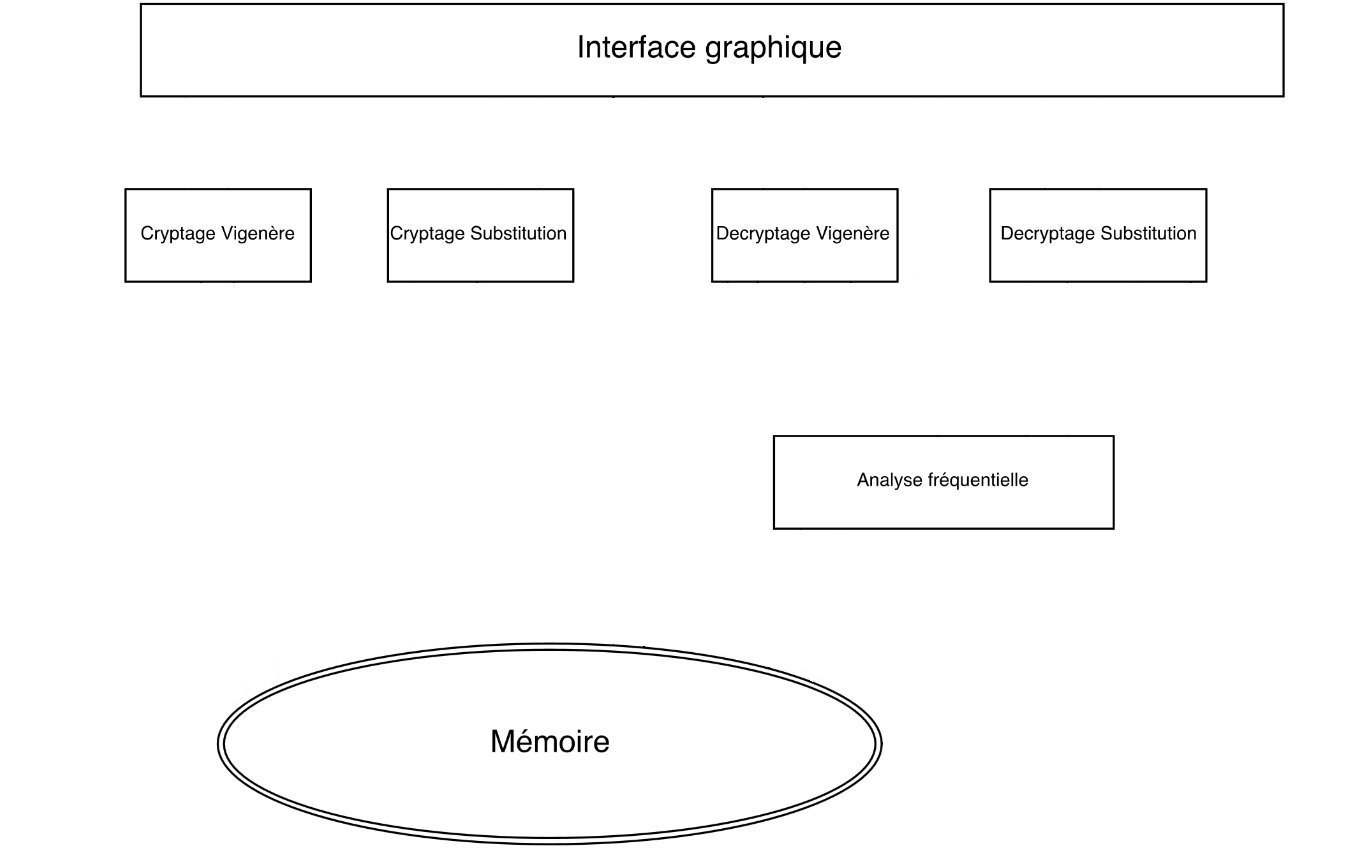
\includegraphics[scale = 0.22]{Org1.jpg}
\end{frame}
\begin{frame}
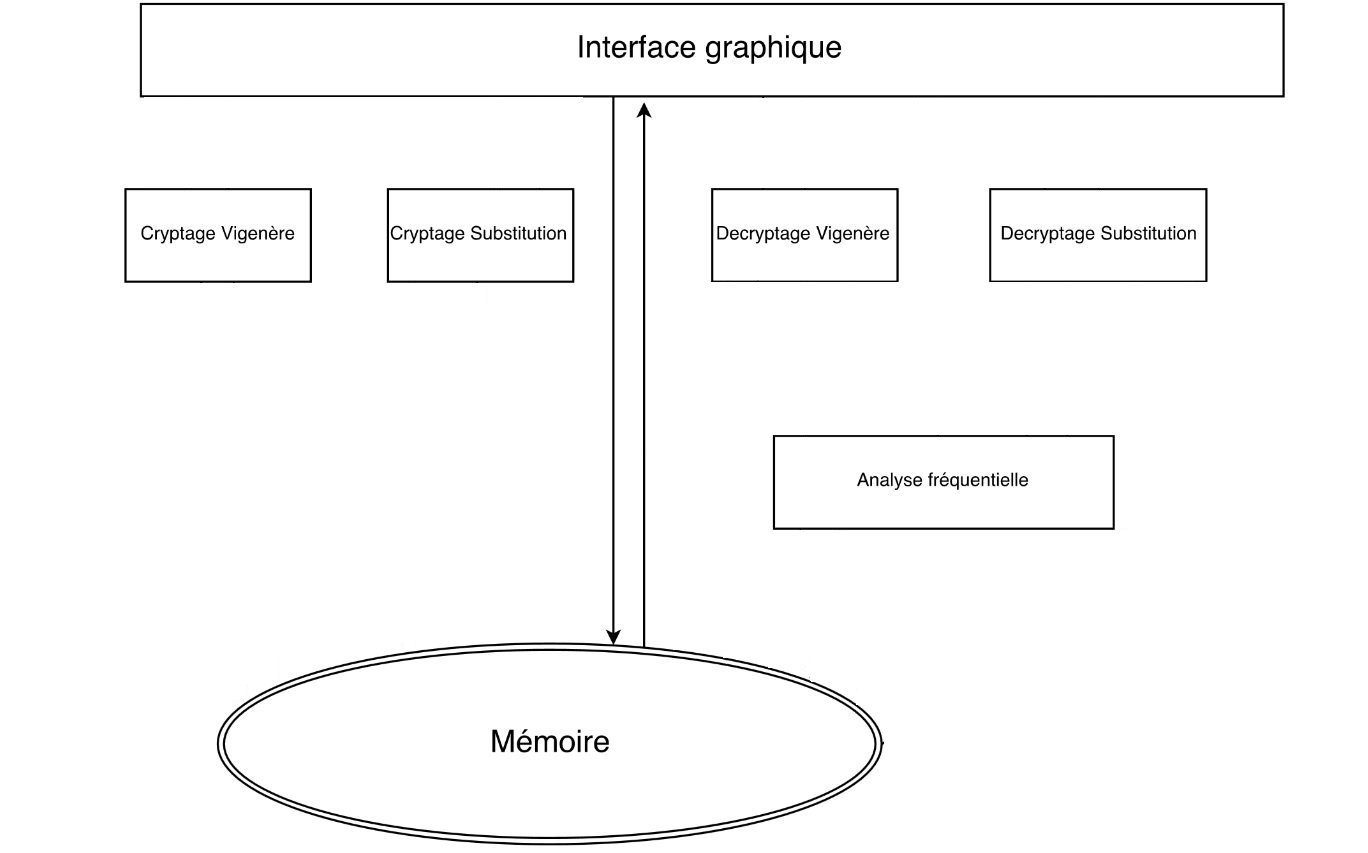
\includegraphics[scale = 0.22]{Org2.jpg}
\end{frame}
\begin{frame}
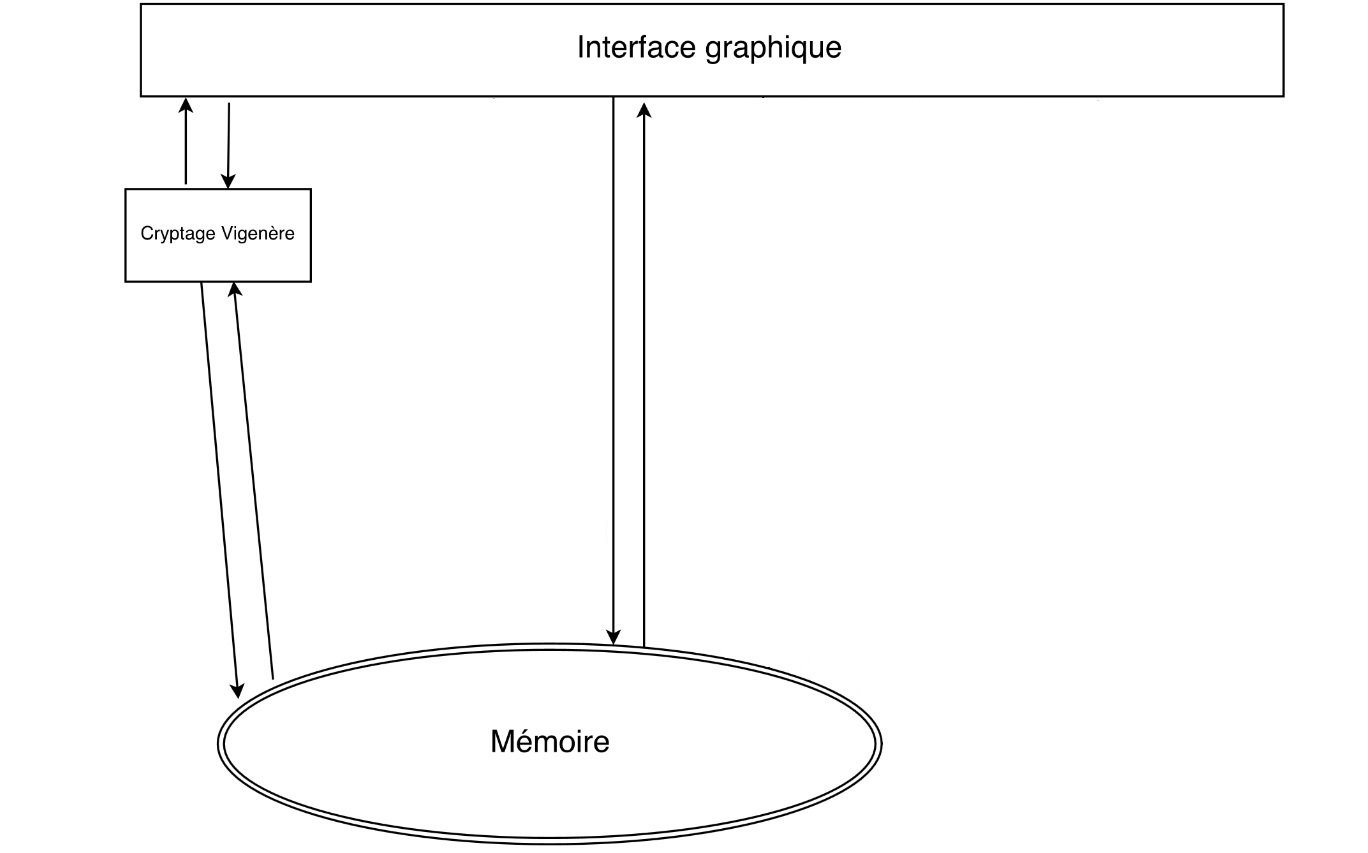
\includegraphics[scale = 0.22]{Org3.jpg}
\end{frame}
\begin{frame}
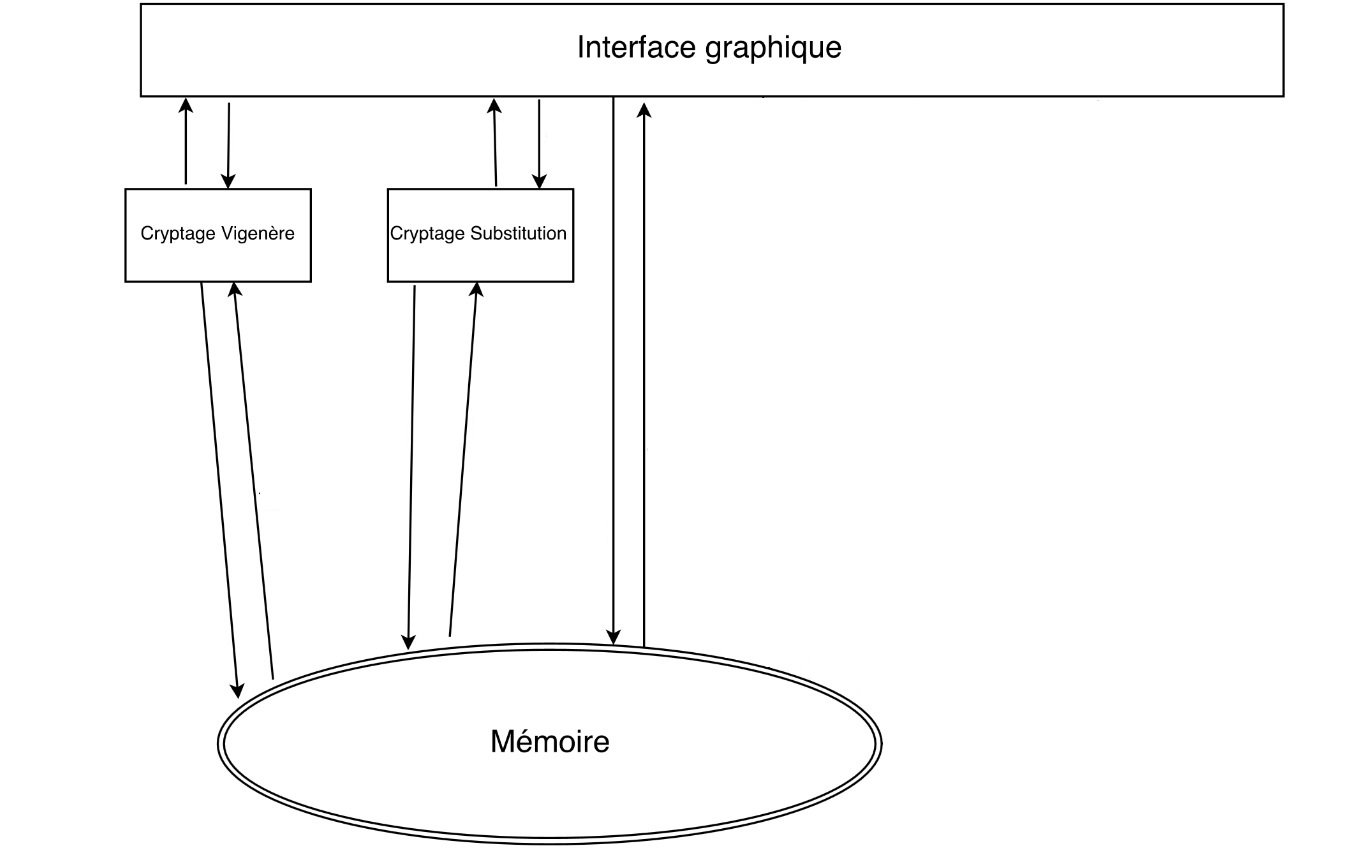
\includegraphics[scale = 0.22]{Org4.jpg}
\end{frame}
\begin{frame}
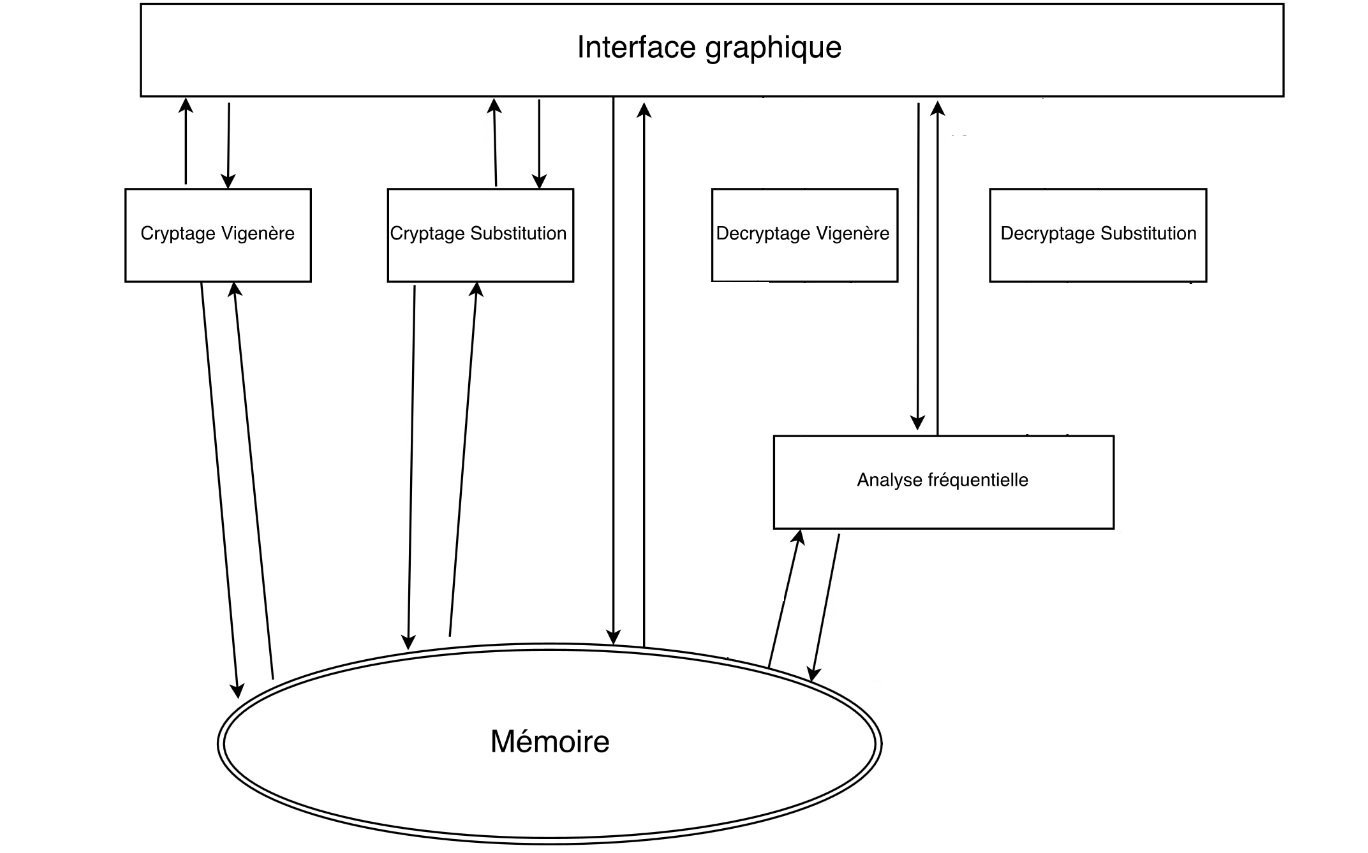
\includegraphics[scale = 0.22]{Org5.jpg}
\end{frame}
\begin{frame}
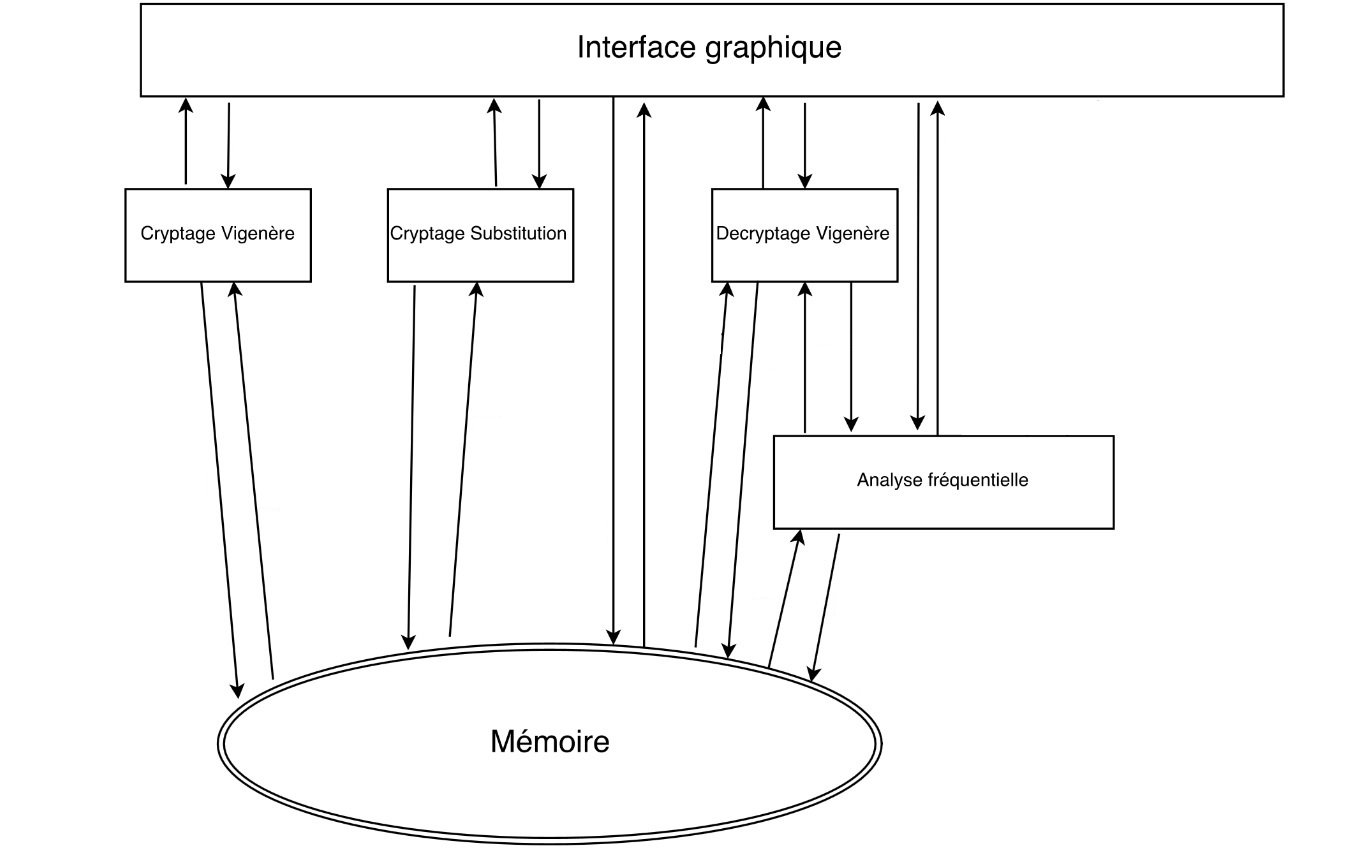
\includegraphics[scale = 0.22]{Org6.jpg}
\end{frame}
\begin{frame}
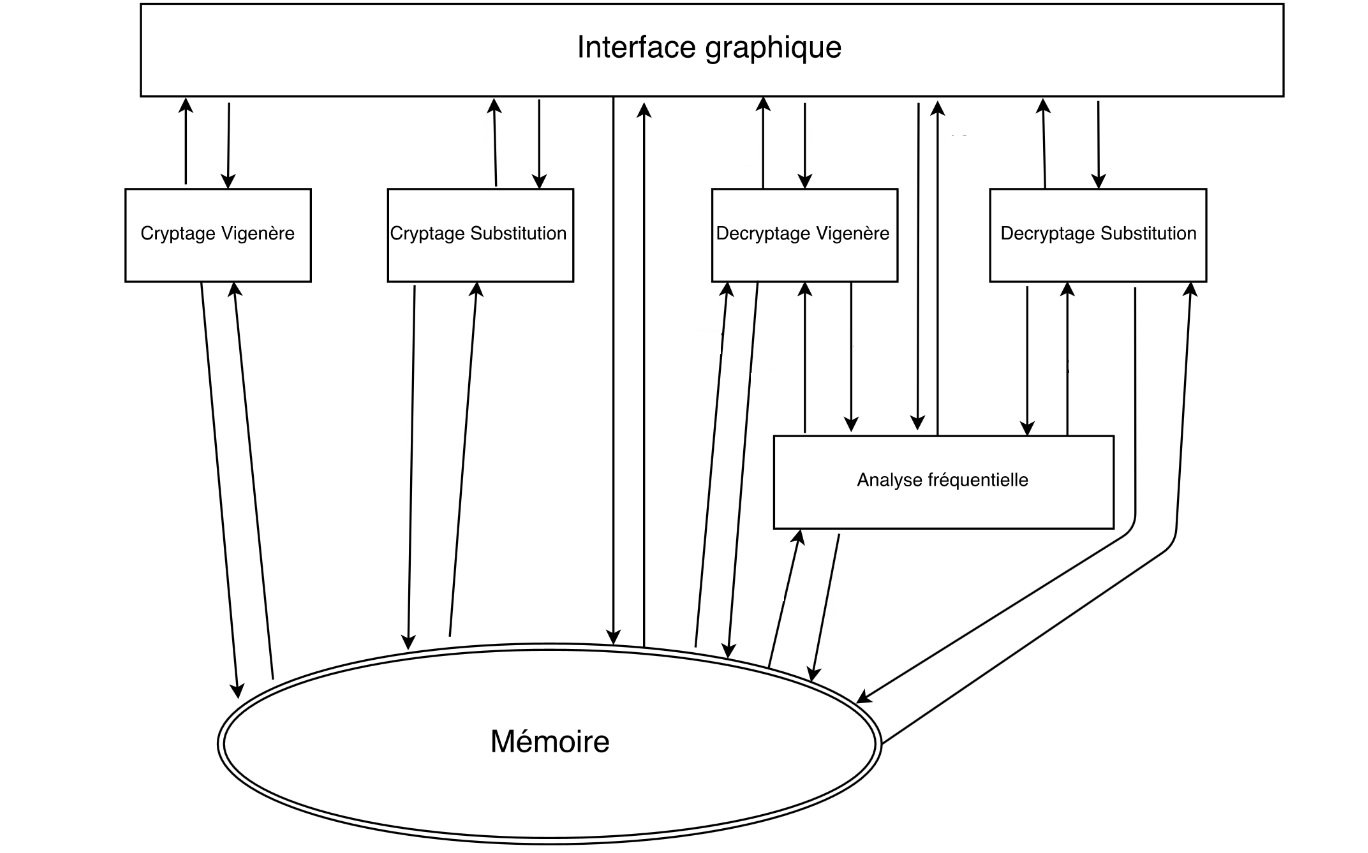
\includegraphics[scale = 0.22]{Org7.jpg}
\end{frame}
%abio
\begin{frame}
	\begin{block}{Hypothèse du coûts en nombre de ligne}
	\begin{center}
		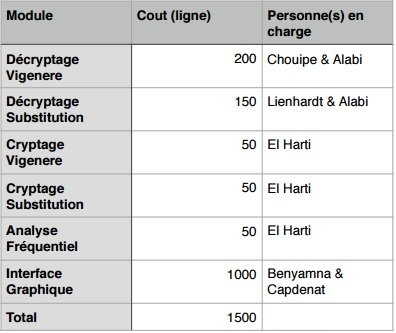
\includegraphics[scale =0.5]{Tableau_cout.jpg} \\ \pause
	\end{center}
	\end{block}
	\begin{block}{Choix du language}
	\begin{itemize}
		\item Language C \\ \pause
		\item Bibliothéque GTK 
	\end{itemize}
	\end{block}
\end{frame}
\begin{frame}
\begin{center}
\Huge {Conclusion}
\end{center}
\end{frame}


\end{document}
